\section{Organigramme du Club Robotronik}

\vspace*{3cm}
\begin{center}
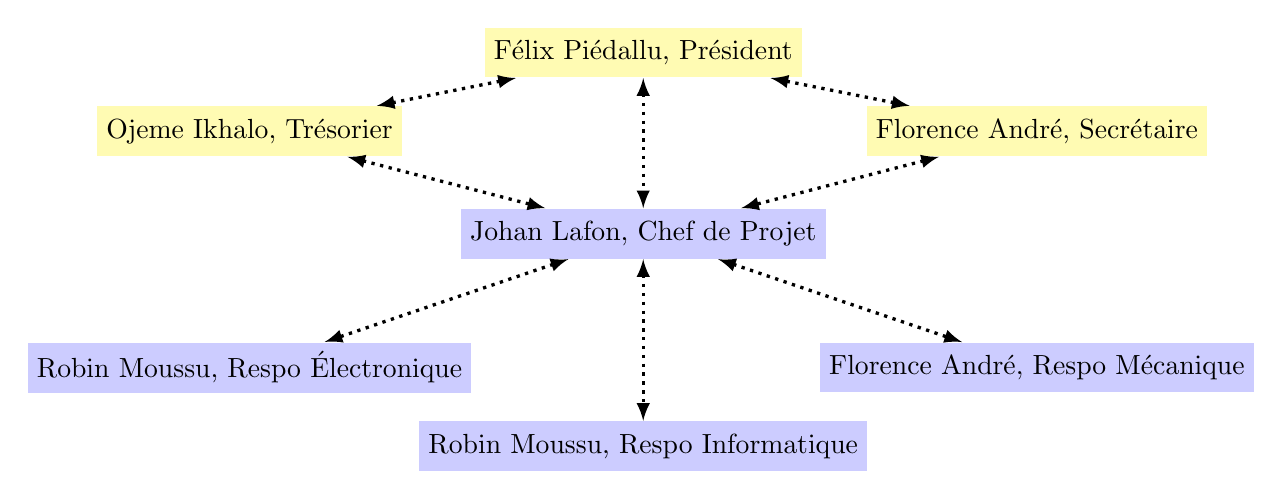
\begin{tikzpicture}
\tikzstyle{bureau}=[rectangle, minimum height=1.8em,fill=yellow!30,text=black]
\tikzstyle{respo}=[rectangle, minimum height=1.8em,fill=blue!20,text=black]
    \node[bureau] (Prez) at (0,0) {Félix Piédallu, Président};
    \node[bureau] (Trez) at (-5,-1) {Ojeme Ikhalo, Trésorier};
    \node[bureau] (Secr) at (+5,-1) {Florence André, Secrétaire};
    \node[respo] (Chef) at (+0,-2.3) {Johan Lafon, Chef de Projet};
    \node[respo] (Elec) at (-5,-4) {Robin Moussu, Respo Électronique};
    \node[respo] (Info) at (+0,-5) {Robin Moussu, Respo Informatique};
    \node[respo] (Meca) at (+5,-4) {Florence André, Respo Mécanique};
    
    
\tikzstyle{ens}=[<->,dotted,very thick,>=latex]
\tikzstyle{sup}=[<->,dotted,very thick,>=latex]
    \draw[ens] (Chef) -- (Meca);
    \draw[ens] (Chef) -- (Info);
    \draw[ens] (Chef) -- (Elec);
    
    \draw[sup] (Trez) -- (Prez);
    \draw[sup] (Secr) -- (Prez);
    
    \draw[sup] (Prez) -- (Chef);
    \draw[sup] (Trez) -- (Chef);
    \draw[sup] (Secr) -- (Chef);
\end{tikzpicture}
\end{center}
\vspace*{7cm}
\begin{figure}[h]
    \begin{flushright}
        Le Président, Félix Piédallu, le 9 Octobre 2014,\\
        
\includegraphics[width=100px]{Public/SignaturePresident}
    \end{flushright}
\end{figure}
